\chapter{Search for Charged Higgs Bosons}\label{chap:hpana}
	This chapter details a search for a charged Higgs boson decaying to a hadronically decaying tau lepton and a neutrino; the phenomenology is discussed in Section \ref{sec:Hpm}. This search contains two subchannels, \taujets and \taulep based on the decay of the  associated top quark in the collision event. The \taujets subchannel ($t\rightarrow Wb, \, W \rightarrow q\bar{q}$)  has a higher branching fraction, leading to higher sensitivity at larger \mHpm values. The \taulep subchannel ($t\rightarrow Wb, \, W \rightarrow \ell \nu$)  has a much lower branching fraction, but takes advantage of single-lepton triggers which enhance background suppression of QCD $\mathrm{jet} \, \rightarrow \, \tau$ fakes. This leads to an increased sensitivity at lower \mHpm values. The extra neutrino in the \taulep decay mode creates extra difficulties in separating signal from background in this subchannel by adding a significant contribution to the \Etm calculation for the event. 

	This chapter discusses in detail the entire analysis, including the signal signatures, event selections, analyzed datasets, modelling of backgrounds, analysis strategy, studies of systematic uncertainties, and results.

	\section{Signature and Event Selection}\label{sec:signal}
		As shown in Figure \ref{fig:hpm-diagrams}, the production of the \Hpm is dependent on the mass \mHpm. Table \ref{tab:hplus-production} shows the production mechanisms for \mHpm values with respect to the top quark mass $m_t$ as well as the main decay mode (and theoretical constraints), as well as the main source of background. The two subchannels have similar signal signatures with a hard scatter source of \Etm, one \tauhad, and at least 1 \bjet from the associated top decay.

		\begin{table}
		\centering
		\caption{\Hpm production mechanisms based on \mHpm, dominant \Hpm decay mode, and the main background associated with the diagram.}
		\resizebox{\textwidth}{!}{
		\begin{tabular}{| c | c | c | c |}
		\hline
		\textbf{\Hpm Mass} & \textbf{Production Mechanism} & \textbf{Decay}  & \textbf{Main Background}\\
		\hline \hline
		\multicolumn{1}{|c|}{\multirow{2}{*}{$\mHpm < m_{t}$}} 		& \begin{tabular}[c]{@{}c@{}} double-resonant $t \rightarrow H^\pm b$ (LO) \\ 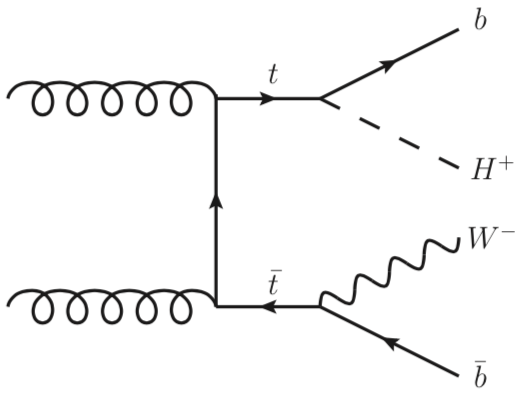
\includegraphics[width=.19\textwidth]{chapters/chapter6_HPlus/images/double_resonant_production_low_mass.png} \end{tabular} 											& \begin{tabular}[c]{@{}c@{}} \HpmLong \\ (low $\tanb \implies$ $\Hpm \rightarrow cs$ or $\Hpm \rightarrow cb$ ) \end{tabular} 																	& \ttbar, single-top \\ \hline

		\multicolumn{1}{|c|}{\multirow{3}{*}{$\mHpm \simeq m_{t}$}} & \begin{tabular}[c]{@{}c@{}} non-resonant $t \rightarrow \Hpm b$ (LO) \\ 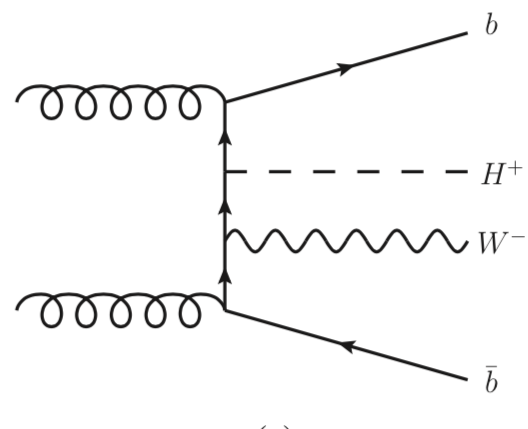
\includegraphics[width=.19\textwidth]{chapters/chapter6_HPlus/images/non_resonant_production_intermediate_mass.png} \\ interferences taken into account \end{tabular} 	& $\Hpm \rightarrow \tau \nu$  																																									& \ttbar, single-top \\ \hline

		\multicolumn{1}{|c|}{\multirow{3}{*}{$\mHpm > m_{t}$}}		& \begin{tabular}[c]{@{}c@{}} single-resonant $gg \rightarrow tbH^\pm$ (NLO) \\ 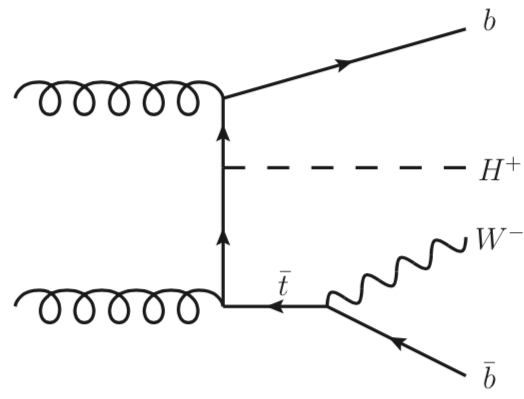
\includegraphics[width=.19\textwidth]{chapters/chapter6_HPlus/images/single_resonant_production_large_mass.png} \end{tabular} 										& \begin{tabular}[c]{@{}c@{}} $\Hpm \rightarrow tb$ \\ ($cos(\beta-\alpha) \simeq 0$ and large $tan(\beta) \implies \Hpm \rightarrow \tau \nu$ \\ $BR(\HpmLong) \simeq 10-15\%$ ) \end{tabular} & multi-jet \\ \hline

		\end{tabular}}
		\label{tab:hplus-production}
		\end{table}

		\subsection{Object Definitions}\label{ssec:object-def}

		  \begin{table}
		  \centering
		  \caption{Definitions of physics objects used in this analysis.}
		  \resizebox{\textwidth}{!}{
		  \begin{tabular}{| c | l | l |}
		  \hline
		  Object & \textbf{\taujets} & \textbf{\taulep} \\
		  \hline \hline
		  \multicolumn{1}{|c|}{\multirow{3}{*}{$\tau$}} & \begin{tabular}[c]{@{}c@{}}Leading reconstructed $\tau$ (regardless of its ID), \\ mediumID$^{*}$, $p_{T} > 40$ GeV, $\abs{\eta}^{***} < 2.3$, $e$ OLR \end{tabular} & \begin{tabular}[c]{@{}c@{}} Leading reconstructed $\tau$ (regardless of its ID), \\ mediumID$^{*}$, $p_{T} > 30$ GeV, $\abs{\eta}^{***} < 2.3$, $e$ OLR \end{tabular} \\[4ex] \hline
		  \multicolumn{1}{|c|}{\multirow{3}{*}{$e$}} & \begin{tabular}[c]{@{}c@{}} LoseLLH, $p_{T} > 20$ GeV, $\abs{\eta}^{***} < 2.47$, \\ Loose isolation, IP cuts \end{tabular} &  \begin{tabular}[c]{@{}c@{}} TightLLH, $p_{T} > 30$ GeV, $\abs{\eta}^{***} < 2.47$, \\ Tight isolation, IP cuts \end{tabular} \\[4ex] \hline
		  \multicolumn{1}{|c|}{\multirow{3}{*}{$\mu$}} & \begin{tabular}[c]{@{}c@{}} LooseID, $p_{T} > 20$ GeV, $\abs{\eta} < 2.5$, \\Loose isolation, IP cuts \end{tabular} & \begin{tabular}[c]{@{}c@{}} TightID, $p_{T} > 30$ GeV, $\abs{\eta} < 2.5$,\\ Tight isolation, IP cuts \end{tabular} \\[4ex] \hline 
		  \multicolumn{1}{|c|}{\multirow{3}{*}{jet}} & \begin{tabular}[c]{@{}c@{}} AntiKt4EMPFlow, $p_{T} > 25$, GeV $\abs{\eta} < 2.5$,\\ JVT$^{**}$  $> 0.59$, Btag=70\%, DL1r \end{tabular} & \begin{tabular}[c]{@{}c@{}} AntiKt4EMPFlow, $p_{T} > 25$ GeV, $\abs{\eta} <2.5$, \\ JVT$^{**}$  $ > 0.59$ , Btag=70\%, DL1r \end{tabular} \\[4ex] \hline
		  \end{tabular}}
		  \label{tab:object-defs}
		  \end{table}

		  % \begin{columns}
		  % \column{.3\textwidth}
		  % \begin{itemize}
		  %   \footnotesize
		  %   \item $\tau$ mediumID$^{*}$
		  %   \begin{itemize}
		  %     \tiny
		  %     \item 1-prong: 75\% ID eff 
		  %     \item 3-prong: 60\% ID eff
		  %   \end{itemize}
		  % \end{itemize}
		  % \column{.3\textwidth}
		  % \begin{itemize}
		  %   \footnotesize
		  %   \item JVT$^{**}$
		  %     \begin{itemize}
		  %       \tiny
		  %       \item $p_{T} < 60$ GeV
		  %       \item $\abs{\eta}<2.4$
		  %   \end{itemize}
		  % \end{itemize}
		  % \column{.3\textwidth}
		  % \begin{itemize}
		  %   \footnotesize
		  %   \item $\abs{\eta}^{***}$
		  %     \begin{itemize}
		  %       \tiny
		  %       \item $1.37 < \abs{eta} < 1.52 $ excluded
		  %   \end{itemize}
		  % \end{itemize}
		  % \end{columns}

		\subsection{Event Selections}\label{ssec:event-selection}

	\section{Datasets}\label{sec:datasets}

		\subsection{Signal Modeling}\label{ssec:sig-modeling}

	\section{Background Modeling}\label{sec:bkg-modeling}

	\section{Analysis Strategy}\label{sec:ana-strat}

		\subsection{Multivariate Analysis Techniques}\label{ssec:mva}

		\subsection{Training}\label{ssec:training}

		\subsection{Feature Selection}\label{ssec:features}

		\subsection{Hyperparameter Optimization}\label{ssec:hpo}

	\section{Systematic Uncertainties}\label{sec:systs}

	\section{Results}\label{sec:results}

